% !Mode:: "TeX:UTF-8"
%% 请使用 XeLaTeX 编译本文.
% \documentclass{WHUBachelor}% 选项 forprint: 交付打印时添加, 避免彩色链接字迹打印偏淡. 即使用下一行:
\documentclass[forprint]{WHUBachelor}
\usepackage{listings}
\lstset{frame=tb,
	language=Java,
	aboveskip=3mm,
	belowskip=3mm,
	showstringspaces=false,
	columns=flexible,
	basicstyle={\small\ttfamily},
	numbers=none,
	numberstyle=\tiny\color{gray},
	breaklines=true,
	breakatwhitespace=true,
	tabsize=4,
	frame=single,
	xleftmargin=2em,
	xrightmargin=2em
}
\usepackage{multirow}
\newcommand{\juhao}{。}
\newcommand{\dunhao}{、}
\begin{document}
%%%%%%% 下面的内容, 据实填

\miji{ }                                      % 密级. 没有就空着.
\StudentNumber{2015301500150} % 填写自己的学号

\title{移动应用的动态行为捕获}
\Etitle{Dynamic behavior capture for mobile applications} % 英文题目
\author{蹇奇芮}                            % 作者名字
\Eauthor{QiRui Jian}            %作者英文名
\Csupervisor{傅建明\quad 教授}        %指导教师中文名、职称
\Esupervisor{Prof.~JianMing Fu}     %指导教师英文名、职称
\Cmajor{信息安全}                  % 专业中文名
\Emajor{Information Security}% 专业英文名
\Cschoolname{国家网络安全学院}          % 学院名
\Eschoolname{School of Cyber Science and Engineering} %学院英文名. 不确定的话, 请看一下自己学院的网页上是怎么写的. 别搞错了!
\date{二〇一九年五月}                    % 日期, 要注意和英文日期一致!!
\Edate{May, 2019}                       % 英文封面日期

%-----------------------------------------------------------------------------
\pdfbookmark[0]{封面}{title}         % 封面页加到 pdf 书签
\maketitle
\frontmatter
\pagenumbering{Roman}              % 正文之前的页码用大写罗马字母编号.
%-----------------------------------------------------------------------------
% !Mode:: "TeX:UTF-8"

%%% 此部分需要自行填写: (1) 中文摘要及关键词 (2) 英文摘要及关键词
%%%%%%%%%%%%%%%%%%%%%%%%%%%%%
%%% -------------  英文封面 (无需改动)-------------   %%%
%%%%%%%%%%%%%%%%%%%%%%%%%%%%%

%%% 郑重声明部分无需改动

%%%---- 郑重声明 (无需改动)------------------------------------%
\newpage
\vspace*{20pt}
\begin{center}{\ziju{0.8}\textbf{\songti\zihao{2} 郑重声明}}\end{center}
\par\vspace*{30pt}
\renewcommand{\baselinestretch}{2}

{\zihao{4}%

本人呈交的学位论文, 是在导师的指导下, 独立进行研究工作所取得的成果,
所有数据、图片资料真实可靠. 尽我所知, 除文中已经注明引用的内容外,
本学位论文的研究成果不包含他人享有著作权的内容.
对本论文所涉及的研究工作做出贡献的其他个人和集体,
均已在文中以明确的方式标明. 本学位论文的知识产权归属于培养单位.\\[2cm]

\hspace*{1cm}本人签名: $\underline{\hspace{3.5cm}}$
\hspace{2cm}日期: $\underline{\hspace{3.5cm}}$\hfill\par}
%------------------------------------------------------------------------------
\baselineskip=23pt  % 正文行距为 23 磅
%------------------------------------------------------------------------------





%%======中文摘要===========================%
\begin{cnabstract}
智能移动终端设备的盛行使得针对移动操作系统的恶意应用迅速增加. 目前的移动操作系统中, 安卓系统巨大的市场份额和其相对开放的应用分发和权限管理方式使得其成为的攻击者的主要目标. 为了识别出恶意应用并阻止其传播, 我们需要对应用的行为进行分析. 然而单纯的静态分析在如今安卓应用成熟的混淆和加壳机制的保护下无法很好的揭示应用的行为, 因此需要动态的对安卓应用的行为进行捕获和分析\juhao 

本文分析了目前已有的一些安卓系统动态分析系统的实现技术, 并且利用hooking技术以及对安卓8.1源代码的修改设计和实现了一个运行于Nexus 5x(Google的一款智能手机)的高性能应用动态行为捕获系统. 该系统能够捕获到Java层的所有方法调用以及本地层的重要函数调用, 并且支持动态地调整需要监控的目标函数(本地层). 本文使用常用应用对该系统进行了测试, 结果显示与同样能捕获到所有java层方法调用的Android Device Monitor\upcite{androidDeviceMonitor}相比本系统的性能开销明显更低\juhao 

本文设计思路结合了hooking技术带来的灵活性和以及修改源代码的稳定性以及高性能, 对其他开源平台的类似工具设计有一定参考作用, 但在应用中应当注意两种方式可能的冲突问题\juhao 




\end{cnabstract}
\par
\vspace*{2em}


%%%%--  关键词 -----------------------------------------%%%%%%%%
%%%%-- 注意: 每个关键词之间用“;”分开,最后一个关键词不打标点符号
\cnkeywords{软件安全; 安卓应用; 动态行为; 恶意软件}


%%====英文摘要==========================%


\begin{enabstract}
Malicious applications on mobile operating systems boom with the prevalence of smart mobile devices. The huge market share of Android, one of current mobile operation systems, and its relatively open application distribution and privilege management make it attackers' major target. In order to identify malicious applications and prevent them from spreading, we need to analyze the behavior of applications. However,  only static analysis can not handle the mature obfuscation and packing mechanism of Android applications, so it is necessary to dynamically capture and analyze the behavior of Android apps.

In this paper, I analyze some existing Android dynamic analysis systems and present a high-performance application dynamic behavior capture system, which can run on Nexus 5x and is implemented by using hooking and modifying Android source code. The system captures all method invocations of Java layer and important function calls of Native layer, and supports dynamic adjustment of the target functions (Native layer) that need monitoring. I evaluate the system with common applications and the result shows that the overhead is significantly lower than that of Android Device Monitor when capturing all java layer method invocations.

The design of the system in ​​this paper combines the flexibility brought by hooking and the stability and high performance brought by modification of source code, which can be used for similar tools on other open source platforms, but we should pay attention to the possible conflicts between the two approaches;

\end{enabstract}
\par
\vspace*{2em}

%%%%%-- Key words --------------------------------------%%%%%%%
%%%%-- 注意: 每个关键词之间用“;”分开,最后一个关键词不打标点符号
 \enkeywords{software security; Android application; dynamic behavior; malware }
    % 加入摘要, 申明.
%==========================把目录加入到书签==============================%%%%%%
\pdfbookmark[0]{目录}{toc}
\tableofcontents
\mainmatter %% 以下是正文
%%%%%%%%%%%%%%%%%%%%%%%%%%%--------main matter-------%%%%%%%%%%%%%%%%%%%%%%%%%%%%%%%%%%%%
\chapter{绪论}
\section{研究背景与意义}
随着移动互联网和物联网的蓬勃发展, 智能移动终端设备迅速普及\juhao 
截止2018年9月,国内智能手机用户数量已达到7.8亿\upcite{smartphone2018statistics}, 占总人口数的55\%以上\juhao 如此众多的用户极大地促进了移动应用的发展, 2018年的数据显示\upcite{appAmount2018}, 谷歌公司的Google Play上已经有超260万应用软件, 苹果公司的App Store上也有超过200万应用软件可供下载使用\juhao 这些应用软件涵盖了娱乐, 社交, 购物, 出行, 金融服务, 身份服务等等领域, 极大地便利了人们的生活\juhao 但与此同时, 各种服务通过应用软件集中于智能手机使得智能手机与个人隐私, 财产安全甚至人身安全的联系变得更加紧密, 从而不可避免地吸引了大量攻击者开发和传播恶意应用来牟取不正当利用\juhao 

目前市场上的智能移动终端设备运行的移动操作系统几乎均为Android和Apple iOS\upcite{mobileOSMarketshare2019}\juhao 其中Android以其免费, 开源的特点吸引了大量智能手机厂商, 占据了超过75\%的市场份额\upcite{mobileOSMarketshare2019}. 最新数据显示, 在2019年Q1国内智能手机销售量中搭载Android的手机销量占比达78.2\%\upcite{mobileOSSalesMarketshare2019}\juhao 然而, Android本身宽松的权限管理以及开放的应用分发方式使其很容易受到攻击, 加上巨大的市场体量, 造成了绝大多数恶意应用把Android作为攻击目标的局面\juhao 虽然近年来Android的权限管理和安全机制不断加强, 同时工信部各大应用分发平台的监管加强, 一定程度上遏制了恶意应用的发展, 但数据显示\upcite{malwareStat}2018年Android新增恶意软件达800.62万个, 感染用户数近1.13亿, 数量仍然庞大\juhao 另外, 恶意软件的类型也持续朝着多样化隐秘化方向发展,新式的恶意软件通过更加难以分析的加壳和混淆技术隐藏自己的恶意行为, 绕过安全软件的查杀\juhao 因此, Android平台的安全问题依然严峻\juhao 

为了阻止恶意应用被下载运行, 保护用户手机的信息安全, 各大应用分发平台需要能够精确有效地判断开发者提交的应用是否为恶意应用, 而捕获应用的行为是分析一个新应用是否为恶意应用的必要前提\juhao 对应用软件的行为获取方法有两个大类: 静态方式和动态方式\juhao 静态方式即在不运行应用软件的情况下对应用软件内部的资源文件、代码、数据等进行分析, 获取应用的特征, 代码逻辑等; 动态方式则是运行应用软件, 在执行过程中对软件的代码执行路径, 数据访问等进行监控和记录\juhao 在目前Android平台的应用加壳和混淆技术成熟的情况下, 单独的静态分析无法获取包含应用的真正逻辑的代码和数据, 因而无法获取到应用行为, 必须通过动态的方式才能捕获到包含应用真实目的的行为, 获取相应的数据, 从而判断应用是否为恶意应用\juhao 另外, 动态分析还能够在运行中捕获到执行应用真正逻辑的代码和数据(脱壳), 从而结合静态分析揭示更加完整的应用行为\juhao 因此, 对Android平台移动应用的动态行为捕获技术进行研究, 有助于识别和分析隐蔽性越来越强的恶意应用, 从而遏制恶意应用的传播, 提升Android平台的安全性\juhao

\section{国内外研究现状和发展方向}
Android系统从发布至今已有10年, 目前国内外已有许多Android应用动态分析相关的研究成果发表\juhao 这些成果借鉴了传统PC平台的动态分析方法, 并结合了Android平台的自身特点, 在本地指令层面, 系统调用层面, 本地函数层面, Java指令层面, Java方法层面中部分或全部层面对应用的运行进行跟踪记录, 并在此基础上结合污点传播技术实现了隐私数据泄露的检测功能, 结合对应用加壳混淆机制的研究实现了脱壳和去混淆功能, 给恶意应用的分析提供了许多强有力的工具\juhao 下文介绍了一些有代表性的成果\juhao

Enck William等构建了名为Taintdroid\upcite{taintdroid}的隐私数据跟踪系统\juhao 该系统采用了污点传播技术, 通过修改Android系统Java层与隐私数据获取相关的API给隐私数据添加标记, 通过修改Android Runtime的Dalvik虚拟机运行机制实现了带标记隐私数据在虚拟机内部的透明传播, 通过修改Android系统进程间通信的接口实现了带标记隐私数据跨进程传播, 通过修改Java层文件和网络的API实现记录带标记的隐私数据去向, 从而能够检测到应用泄露隐私数据的行为\juhao 不过该系统有以下局限性: 
1. 没有对应用的所有敏感行为进行监控, 例如拨打电话, 发送短信等\juhao
2. 没有对Native层的函数进行监控, 无法检测到应用通过JNI接口调用自身Native模块泄露隐私数据的行为\juhao
3. 针对特定Android版本, 并且不再支持Android4.3以后的版本使用\juhao
 
Desnos Anthony等构建了名为Droidbox的\upcite{droidbox}动态分析系统\juhao 该系统使用了Taintdroid\upcite{taintdroid}来监控隐私数据泄露, 另外通过修改Android系统源代码中敏感API的方式实现对Java层的电话, 短信, 网络, 文件, Java类动态加载, 加密等API调用的监控, 能够记录应用在Java层的敏感行为\juhao 但该系统只涉及了Java层预定义的敏感API的监控, 没有实现对应用本地函数层调用的监控, 因此无法完整的揭示应用的行为, 另外该系统也针对特定Android版本开发, 并且不支持Android4.1之后的系统使用\juhao

Google公司构建了名为Bouncer\upcite{googlebouncer}的恶意应用检测系统\juhao 该系统利用静态分析的方式识别已知的恶意软件, 同时通过动态分析方式使用虚拟机运行应用并记录其行为, 从而判断其是否为恶意应用\juhao

Yan Lok Kwong等构建了名为DroidScope\upcite{droidscope}的动态分析系统\juhao 该系统通过修改运行Android系统的qemu虚拟机以及运行的Android系统来实现, 提供了对本地指令层面和Java指令层面的


\section{论文主要工作}
本文分析了目前已有的一些安卓系统应用行为监测系统的实现方式和优缺点, 并且通过hook技术以及对安卓8.1源代码的修改设计和实现了一个运行于Nexus 5x(Google的一款智能手机)的高性能应用动态行为捕获系统. 该系统能够捕获到Java层的所有方法调用以及Native层的重要函数调用, 并且支持动态地调整需要监控的目标方法(Java层)和函数(Native层). 本文使用常用应用对该系统进行了测试, 结果显示与同样能捕获到所有java层方法调用的Android Device Monitor相比本系统的性能开销明显更低.

\section{论文组织结构}
根据本文研究的特点, 本文的内容按如下方式组织:

第一章为绪论, 主要说明了本文课题的研究背景, 研究意义, 简述了国内外对本文课题的研究现状及发展方向, 介绍了本文的主要工作内容和文章组织结构\juhao 

第二章为背景技术介绍, 主要讲述了Android系统的基本架构, Android应用的基本结构, Android平台的常用动态分析技术和应用保护技术, Android Runtime的运行机制和Frida框架\juhao

第三章为系统设计和实现, 详细说明了本文提出的监控系统的原理与组成结构\juhao

第四章为实验与结果分析, 描述了实验环境, 实验方法并对实验结果进行了分析和总结\juhao

第五章为总结与展望, 主要是整理本文所做的工作,并简要分析了本文提出系统的局限性和改进方案\juhao

 
\chapter{背景技术分析}
\section{Android系统架构}
Android系统由多个软件层次构成, 这些层次功能分明, 每一层都对其上的一层提供服务, 构成一个5层的软件栈\juhao 软件栈最底层为Linux内核层, 其上为硬件抽象层, 之后为本地函数库层, 该层次包括了Android Runtime和其他的一些本地函数库, 再上层为Android框架层, 该层包括了提供给应用程序的API和系统管理服务程序, 最上层为应用层, 该层次为用户直接交互的应用程序运行的层次\juhao  图\ref{androidStructure}给出了各层次的组件和关系\juhao
\begin{figure}[ht]
\centering
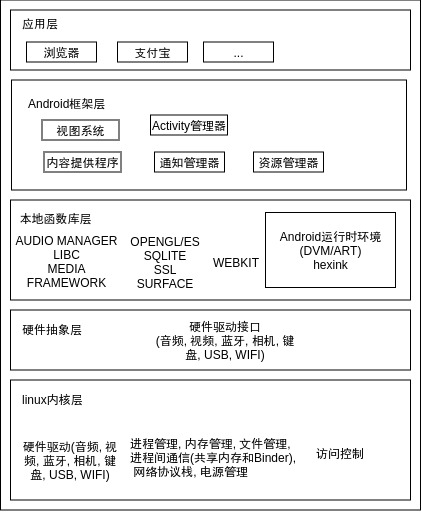
\includegraphics[width=\textwidth]{android_structure.jpg}
\caption{Android系统架构}
\label{androidStructure}
\end{figure}

\subsection*{Linux内核层} 
Android基于修改的Linux内核构建, Linux内核为Android系统提供了操作系统的基本功能, 包括进程管理, 内存管理, 文件管理, 进程间通信(共享内存和Binder), 网络协议栈, 电源管理, 许多设备驱动程序(音频, 视频, 蓝牙, 相机, 键盘, USB, WIFI等)以及访问控制机制(基于用户和用户组的访问控制和selinux)\juhao 这些功能通过系统调用的方式提供给上层使用, 因此, 监控系统调用的使用情况能够获取到应用对关键资源的访问行为\juhao

\subsection*{硬件抽象层}
硬件抽象层是定义了用于更高层次调用对应硬件驱动的接口, 屏蔽了不同厂商的同种设备驱动的差异, 降低Android系统与硬件的耦合度, 便于Android系统的移植\juhao 硬件抽象层包含多个库模块,其中每个模块都为特定类型的硬件组件实现一个接口,例如相机或蓝牙模块。当更高层次要求访问设备硬件时,Android系统将为该硬件组件加载库模块。

\subsection*{本地库层}
本地库层由许多由C/C++开发的系统运行库组成\juhao 这些运行库主要分为两部分, 第一分部为Android运行时环境相关的库, 第二部分为其他系统运行库\juhao 

Android运行时环境由给应用提供Java运行环境的虚拟机实现和实现Java API的核心运行时库组成\juhao 虚拟机实现在Android4.4之前为Dalvik虚拟机, Android4.4时ndroid Runtime(ART)虚拟机作为实验特性加入, 并喝Dalvik虚拟机共存, Android5.0之后只保留了ART虚拟机\juhao Android框架层的许多服务程序和应用层的应用软件就运行在自身的虚拟机实例中\juhao 核心运行时库,可提供Java API框架使用的Java编程语言大部分功能\juhao

其他系统运行库包括许多重要的功能的实现, 主要包括以下部分: 
AUDIO MANAGER用于管理音频输入输出; 
LIBC提供了c语言标准函数库; 
MEDIA FRAMEWORK提供了对常见音频和视频处理的支持; 
OPENGL/ES提供了2D/3D图形绘制功能;
SQLITE提供了访问SQLite数据库的函数;
SSL提供了常见的加密功能;
SURFACE MANAGER提供对显示子系统的支持和管理;
WEBKIT提供了浏览器引擎的实现\juhao

本地库层的各种功能函数除了提供给Android系统自身以实现系统服务功能, 还可以通过Android Native Development Kit(NDK)让应用程序通过Java Native Interface(JNI)调用, 因此对本层函数调用情况的监控可以获取到应用的行为\juhao

\subsection*{Android框架层}
Android框架层包括了许多系统服务程序和组件以及提供给应用程序的访问系统资源的Java API\juhao 这些服务程序和组件主要包括以下几部分:

1. 资源管理器,用于访问非代码资源,例如本地化的字符串、图形和布局文件

2. 通知管理器,可让所有应用在状态栏中显示自定义提醒

3. Activity管理器,用于管理应用的生命周期,提供常见的导航返回栈

4. 内容提供程序,可让应用访问其他应用(例如“联系人”应用)中的数据或者共享其自己的数据

5. 丰富、可扩展的视图系统,可用以构建应用的 UI,包括列表、网格、文本框、按钮甚至可嵌入的网络浏览器

Android框架层是与应用程序联系最紧密的层次, 也是应用程序最容易访问系统资源的层次, 因此对该层次提供的API的监控能够显示应用的主要行为\juhao

\subsection*{应用层}
应用层包括了所有用户直接使用的应用软件,例如电话、短信、浏览器、微信、支付宝等\juhao 这些应用软件主要由Java语言开发, 通过调用Android框架层提供的API和Java语言的标准API实现功能, 每个应用运行于自己独立进程中的虚拟机实例中, 多个应用间借助框架层提供的API通信(进程间通信最终由内核实现)\juhao 利用NDK, 应用也可以实现自己的本地库, 访问Android系统本地库层的开放甚至隐藏的函数, 并通过JNI在应用的Java部分调用自身的本地库中的本地函数\juhao 由于应用能够直接执行本地代码, 增加了应用程序行为涉及的层次, 需要同时在Java层次和本地层次监控应用的执行才能获取到应用的所有行为\juhao


\section{Android应用结构}
\subsection{应用安装包结构}
Android应用程序主要以Android Package(APK)的文件形式分发和安装\juhao APK文件本质上是一种zip压缩文件, 由多个文件和文件夹组成 其中包含了应用的代码文件、资源文件、证书文件和清单文件, 以apk作为文件后缀名\juhao 图\ref{packageStructure}给出了APK文件的内部结构\juhao
\begin{figure}[ht]
	\centering
	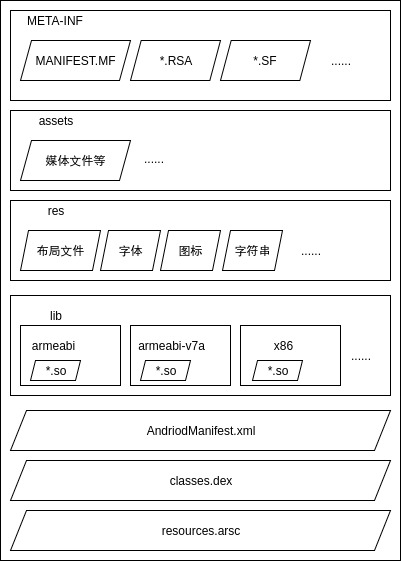
\includegraphics[width=8cm]{package_structure.jpg}
	\caption{APK文件结构}
	\label{packageStructure}
\end{figure}

META-INF文件夹包含了与APK文件的签名和校验相关的文件, 一般应该包括至少3个文件:MANIFEST.MF、*.RSA、*.SF(“*”表示文件名不确定)\juhao 
其中MANIFEST.MF记录了APK中的所有文件名和经过base64编码的SHA256校验值(不包括自身);
*.SF记录了MANIFEST.MF文件的经过base64编码的SHA256校验值以及MANIFEST.MF中每一项记录的经过base64编码的SHA256校验值;
*.RSA文件中保存了公钥、所采用的加密算法以及对CERT.SF中的内容的用私钥进行加密之后的值\juhao

assets文件夹包括了res中定义类型之外的其他类型的资源文件,例如音频文件,视频文件等媒体文件\juhao 该文件夹内的文件不会被编译处理, 因此可以放入任意格式的文件, 应用甚至可以把本地库文件放在这个文件里在运行时根据需要动态的加载\juhao

res文件夹内包含了除了字符串外其他较复杂资源文件, 例如布局文件, 字体文件, 图标文件, 颜色文件等\juhao 这些文件会在应用运行时根据resources.arsc中记录的资源ID对应的路径进行调用\juhao

lib文件夹包括了应用的本地库文件, 根据适用的Application Binary Interface(ABI)不同,这些本地库文件会被放在不同的子文件夹里\juhao 当APK被安装时, 系统会选择合适的本地库文件进行安装, 在启动应用时系统会自动加载对应的本地库文件\juhao

AndroidManifest.xml文件是重要的清单文件, 描述了应用的组件以及其他的一些配置, 通过该文件能够获取到应用的许多基本信息, 具体来说包含以下几个方面:

1.记录了应用软件的名称, 该名称独一无二用于识别该应用;

2.记录了应用的所有组件, 包括构成应用的 Activity、服务、广播接收器和内容提供程序, 以及这些组件可以处理的Intent消息;

3.描述了应用需要使用的权限;

4.声明了应用运行所需的最低Android API级别(与Android版本相对应)

5.列出应用必须链接到的本地库

classes.dex文件为应用的Java代码编译后的运行于ART或者Dalvik虚拟机的可执行文件\juhao 该文件包含了应用自定义的类的实现代码, 通过反编译该文件可以得到应用的Java源代码, 因此通常会使用加壳和混淆的手段隐藏该文件真正的内容\juhao 对于大型应用, 可能会有多个dex文件, 命名为classes2.dex、classes3.dex等\juhao

resources.arsc文件为资源文件索引文件, 其本身包含了全局常量字符串以及其他较复杂资源的路径, 系统正是通过该文件来访问res中的其他资源文件的\juhao 通过修改该文件中其他资源对应的路径可以隐藏res文件夹, 从而隐藏其他资源文件\juhao

\subsection{应用组织结构}
Android应用的功能主要由四种组件实现, 这四种组件为Activity、服务、内容提供程序、广播接收器\juhao 这些组件可能会存在相互依赖的情况,但每个组件都以独立实体形式存在,发挥特定作用, 能够被单独的调用\juhao 各组件的具体功能如下:

Activity表示一个用户能够直接交互的界面\juhao 例如,电子邮件应用可能具有一个显示新电子邮件列表的Activity、一个用于撰写电子邮件的Activity以及一个用于阅读电子邮件的Activity。 尽管这些 Activity 通过协作在电子邮件应用中形成了一种紧密结合的用户体验,但每一个 Activity 都独立于其他 Activity 而存在。 因此,其他应用可以启动其中任何一个 Activity(如果电子邮件应用允许)\juhao 例如,相机应用可以启动电子邮件应用内用于撰写新电子邮件的 Activity,以便用户共享图片\juhao

服务是一种在后台运行的组件,没有用户界面, 用户无法直接与之交互, 常用于执行长时间运行的操作或为远程进程执行作业\juhao 例如,当用户位于其他应用中时,服务可能在后台播放音乐或者通过网络获取数据,但不会阻断用户与 Activity 的交互。 诸如 Activity 等其他组件可以启动服务,让其运行或与其绑定以便与其进行交互\juhao

内容提供程序管理一组共享的应用数据\juhao 应用数据可以被存储在文件系统、SQLite 数据库、网络上或任何应用可以访问的永久性存储位置, 其他应用可以通过内容提供程序查询数据,甚至修改数据(如果内容提供程序允许)\juhao 例如,Android 系统可提供管理用户联系人信息的内容提供程序。 因此,任何具有适当权限的应用都可以查询内容提供程序的某一部分(如 ContactsContract.Data), 以读取和写入有关特定人员的信息\juhao
内容提供程序也适用于读取和写入您的应用不共享的私有数据\juhao 例如,记事本示例应用使用内容提供程序来保存笔记\juhao

广播接收器是一种用于响应系统范围广播通知的组件\juhao 许多广播都是由系统发起的, 例如,通知屏幕已关闭、电池电量不足或已拍摄照片的广播\juhao 应用也可以发起广播, 例如,通知其他应用某些数据已下载至设备,并且可供其使用\juhao 尽管广播接收器不会显示用户界面,但它们可以创建状态栏通知,在发生广播事件时提醒用户\juhao 但广播接收器更常见的用途只是作为通向其他组件的“通道”,例如,它可以在接收到某个事件广播后启动一项服务来执行某项工作\juhao

\section{Android运行时环境}
\label{androidRuntime}
Android运行时环境本质上是一个虚拟机, 用于执行Android应用中dex文件内的字节码, Android应用和许多Android系统服务都运行在Android运行时环境中\juhao 从2008年第一个Android版本发布至今, Android运行时环境经历了许多变化, 其中最大的变化是从Android4.4前的Dalvik虚拟机变成了Android5.0之后的ART虚拟机\juhao 下面的内容将会根据Android8.1的ART虚拟机从应用启动\dunhao 类的加载\dunhao 方法的执行\dunhao 三个方面分析应用在Java层执行流程\juhao

\subsection{应用的启动}
Android系统中有一个十分重要的进程叫做Zygote, 大多数应用进程和系统进程都是由Zygote产生的\juhao 图\ref{zygoteStart}描述了Zygote进程的启动过程\juhao
\begin{figure}[ht]
	\centering
	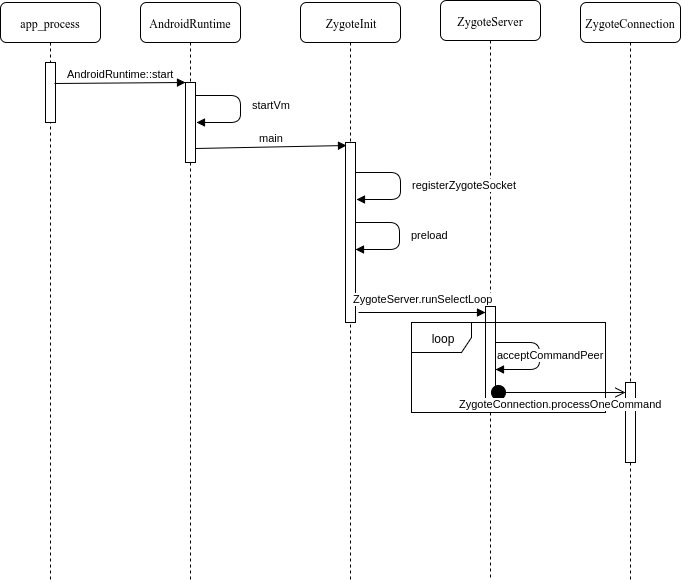
\includegraphics[width=\textwidth]{zygote_start.jpg}
	\caption{Zygote进程启动过程}
	\label{zygoteStart}
\end{figure}

首先系统会启动/system/bin目录下的本地程序app\_process, app\_process解析自身参数后若发现参数中有--zygote就会将进程名改为Zygote然后调用AndroidRuntime::start启动Android运行时环境, 并把入口类设置为com.android.internal.os.ZygoteInit\juhao 进入AndroidRuntime后, 会调用startVM启动ART虚拟机, 之后就会开始执行上述入口类ZygoteInit的main方法\juhao 该类的main方法中首先调用registerZygoteSocket注册一个socket用于之后从该socket接收创建应用进程的命令并执行, 然后会调用preload加载许多重要的类, 最后会调用ZygoteServer.runselectLoop进入一个死循环\juhao 至此, Zygote进程就启动完成了\juhao 在runselectLoop的死循环中, 其会调用acceptCommandPeer等待创建应用的命令, 接收到命令后调用ZygoteConnection.processOneCommand使用fork机制来创建新进程, 所以Zygote在启动后会一直执行runselectLoop直到关机\juhao

了解了Zygote进程的启动过程后, 下面是Android应用的启动过程\juhao Android应用是通过四大组件构成的, 这里通过启动一个Activity的过程来介绍应用的启动过程\juhao 图\ref{appStart}和\ref{appStart2}描述了启动一个没有运行的应用的过程(省略了一些不需要关心的调用过程)\juhao
\begin{figure}[ht]
	\centering
	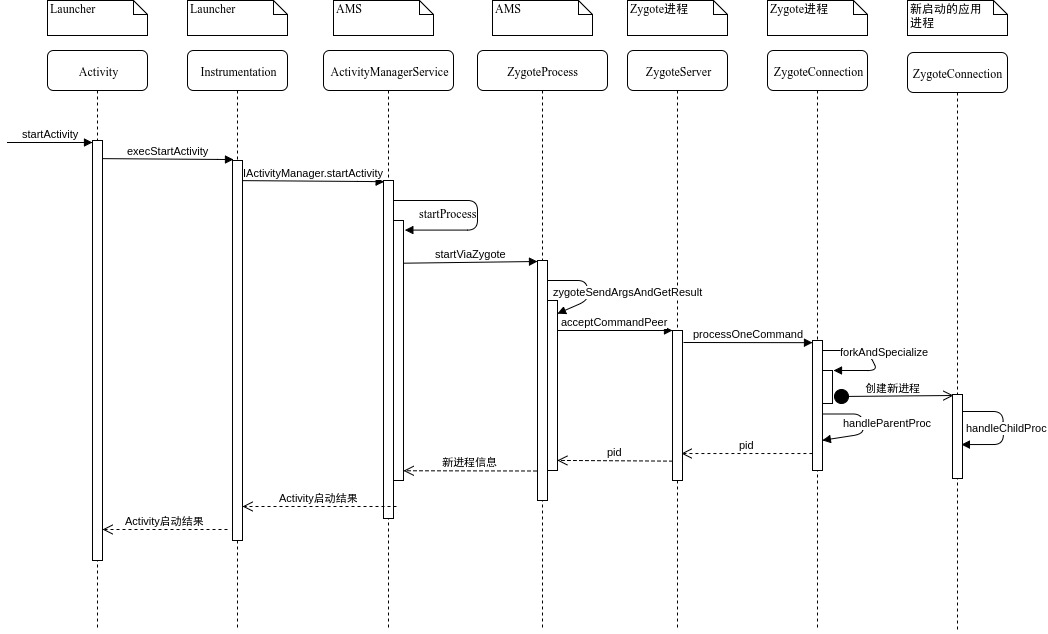
\includegraphics[width=\textwidth]{app_start.jpg}
	\caption{应用启动过程-1}
	\label{appStart}
\end{figure}

\begin{figure}[ht]
	\centering
	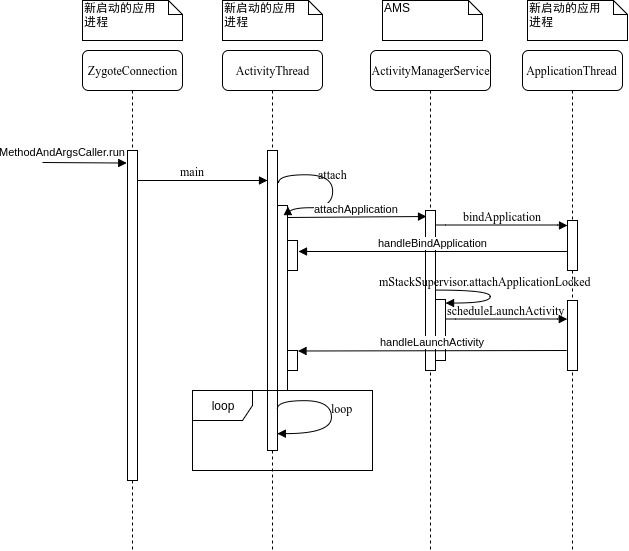
\includegraphics[width=\textwidth]{app_start2.jpg}
	\caption{应用启动过程-2}
	\label{appStart2}
\end{figure}
首先启动器调用Activity类的startActivity方法用于启动一个Activity, 该方法又会调用Instrumentation类的execStartActivity方法; execStartActivity通过Binder机制远程调用系统服务ActivityManagerService(AMS)的startActivity方法来创建Activity\juhao 由于应用还没有启动, AMS会调用startProcessLocked来创建新应用的进程, 该方法最终会调用ZygoteProcess类的zygoteSendArgsAndGetResult方法通过在介绍Zygote进程启动部分提到的socket方法参数来然Zygote进程生成一个新的应用进程\juhao Zygote进程接收到创建新进程的命令后执行forkAndSpecialize方法产生一个新的进程, 并把该进程pid返回给AMS\juhao 新创建的进程通过handleChildProc来做一些初始化操作, 比如关闭Zygote进程的socket, 之后会找到android.app.ActivityThread类并开始执行其main函数\juhao



\subsection{类的加载}


\subsection{方法的执行}


\section{Android动态分析相关技术和实现工具}
Android平台的动态分析同传统PC环境有相似之处, 即都是通过追踪应用软件的控制流和数据流实现对应用软件行为的揭示\juhao 但Android系统的多层次架构使得动态分析系统需要能够同时对本地层和Java层对应用的执行进行监控才能够获取到应用的完整行为\juhao 对各层次的监控, 常用的技术如下:

\subsection{Virtual Machine Introspection}
Virtual Machine Introspection(VMI)是一种实时监控虚拟机运行状态的技术\juhao 通过该技术, 能够实现在指令层面监控应用的运行, 因此也可以实现对系统调用, 本地函数调用的监控\juhao 并且由于监控代码运行于客户系统之外, 客户系统内被监控的应用无法检测到自己处于被监控状态, 因此是一种十分有效的监控应用运行的技术\juhao 对于Android平台的动态监控而言, 使用VMI技术无需修改Android源代码, 可以适应Android版本的变化, 但该技术的运用依赖于模拟器, 一般通过修改模拟器加入监控代码来实现, 但由于依赖模拟器, 容易受到应用对模拟器环境检测的影响\juhao Cooperdroid\upcite{copperdroid}、DroidScope\upcite{droidscope}使用了该技术来实现动态监控\juhao

\subsection{ptrace系统调用}
ptrace系统调用是Unix和一些类Unix系统中的一种系统调用\juhao 通过使用ptrace系统调用, 一个进程可以监控另外一个进程的执行, 读取和修改其内存和寄存器\juhao 具体来说, ptrace系统调用能够实现监控应用调用系统调用的情况, 能够实现指令单步执行和断点, 许多调试工具都依赖于ptrace系统调用实现, 如gdb, lldb, strace, ltrace等\juhao 由于ptrace系统调用能够实现单步执行, 通过ptrace系统调用也能实现在指令层面监控应用的执行\juhao 加上ptrace系统调用能够监控应用调用系统调用的情况, 通过ptrace系统调用可以实现对本地函数调用的监控\juhao 对于Android平台的动态监控而言, 使用ptrace系统调用也无需修改Android源代码, 可以适应Android版本的变化, 并且相比VMI技术, ptrace系统调用不依赖于模拟器, 可以运行于真机上, 但存在一些反ptrace跟踪的技术, 例如一个进程只能被一个进程跟踪, 所以应用可以跟踪自身, 从而防止被其他工具跟踪\juhao ptrace系统调用一般还会和hooking技术结合起来使用, 可以实现对目标函数的劫持和监控\juhao Crowdroid\upcite{crowdroid}\dunhao Glassbox\upcite{glassbox}使用了该技术来实现动态监控\juhao

\subsection{Application Instrumentation}
Application Instrumentation指通过修改需要监控的目标应用, 向其中插入监控代码实现监控应用执行的技术\juhao 对于Android平台而言, 该技术一般用于监控应用调用Java层API的情况, 具体来说, 通过反编译应用的dex文件得到smali代码, 搜索其中调用敏感API的代码, 将监控代码插入调用敏感API代码的周围, 再将修改后的smali代码编译重新打包成包含监控代码的应用, 这样在应用执行时就会执行监控代码, 输出监控信息\juhao 该技术不需要修改Android系统源代码, 但受到Android系统API变化的影响, 因此会在一定程度上受Android版本变化的影响\juhao 此外, 由于应用完整性校验以及加壳和混淆技术的广泛应用, 修改后的应用很可能无法运行, 并且一般无法从应用安装包获取到包含应用真实逻辑的dex文件, 因此该技术目前几乎已经失效\juhao APIMonitor\upcite{apimonitor}使用了该技术实现动态监控\juhao

\subsection{DVM/ART Instrumentation}
DVM/ART Instrumentation指通过修改Android系统的DVM或者ART运行时环境, 在关键的部分加入监控逻辑实现监控应用在Java层执行情况的技术\juhao 一般来说, 可以修改Android运行时环境中方法执行相关的函数来实现对应用执行的方法以及其参数和返回值的监控, 也可以修改Android运行时环境中的字节码解释器实现对Java层指令级别的监控, 在\ref{androidRuntime}节有关于Android运行时环境更详细的描述\juhao 该方法有些类似于上面提到的VMI技术, 在虚拟机层面监控虚拟机内部运行的应用, 在实现全面监控应用运行的同时也使得应用无法检测到自己处于受监控状态, 因此是监控应用Java层行为的一种十分有效的技术\juhao 并且该技术不依赖于模拟器, 利用其开发的动态监控系统可以运行于真机上, 不受应用检测模拟器机制的影响\juhao 但该技术的实现依赖于对
Android源代码的修改, 并且Android运行时环境在不同版本上变化较大, 特别是Android5.0之前和Android5.0之后Android运行时环境有DVM替换为了ART, 因此需要经常调整以适用于最新的Android版本\juhao DroidScope\upcite{droidscope}\dunhao Glassbox\upcite{glassbox}使用了该技术实现动态监控\juhao

\subsection{Hooking技术}
hooking技术是一类劫持函数调用的技术, 通过hooking技术, 我们可以获取目标函数的参数和返回值, 可以改变目标函数的行为从而实现对目标函数的监控\juhao 对于Android平台, hooking技术可以用于监控本地函数也可以用于监控Java方法, 其具体的实现方式有很多种, 例如针对本地函数有Procedure Link Table(PLT) hooking\dunhao inline hooking\dunhao Import Address Table(IAT) hooking; 针对Java方法有修改vtable, 修改ArtMethod对象的入口地址等\juhao hooking技术一般比较灵活, 结合一些动态代码追踪工具, 例如frida, 能够动态的调整监控目标\juhao 由于ptrace系统调用能够修改被追踪进程的内存, linux系统的hooking技术一般会利用ptrace系统调用实现\juhao REAPER\upcite{reaper}使用了该技术实现动态监控\juhao

\subsection{Frida}
Frida是一个著名的开源hook框架\juhao

\subsection{Xposed}

\subsection{Valgrind}

\section{Android应用加固技术}
为保护知识产权, 防止逆向分析, 许多Android应用都采用了加固技术来保护自己的代码, 目前常用的技术包括名称混淆\dunhao 方执行混淆\dunhao dex文件动态加载\dunhao dex文件动态修改\dunhao 类动态加载\dunhao 方法本地实现\dunhao 模拟器检测\dunhao 反调试等\juhao

\paragraph*{名称混淆}
该技术即在应用发布时按照一定的规则将开发应用时定义的有意义的类名\dunhao 方法名\dunhao 和变量名替换称无意义的字符, 从而增加了逆向分析方法用途的难度\juhao

\paragraph*{方法执行混淆}
该技术通过hooking技术使用将一个方法的代码用另外一个方法替换从而使得动态监控系统记录的方法调用和实际的方法调用不同, 因此能够隐藏应用行为, 极大地增加了动态分析的难度\juhao

\paragraph*{dex文件动态加载}
该技术通过先将包含应用真实逻辑的dex文件加密, 在应用运行时再调用解密代码释放dex文件并动态加载来实现隐藏包含应用真实逻辑的dex文件\juhao 该技术用于对抗静态分析十分有效, 可以使得静态分析无法获取到应用的真实逻辑\juhao

\paragraph*{dex文件动态修改}
该技术为dex文件动态加载技术的改进\juhao 采用该技术时, 加载到内存的dex文件并不完全解密, 而是在具体的方法调用前修改方法对应dex文件中的部分为方法的真正指令, 在方法执行后又抹去对应指令\juhao 该技术用于对抗一些Android平台的脱壳工具, 使其无法得到完整的dex文件\juhao

\paragraph*{类动态加载}
该技术把类方法的字节码分散到多个dex文件中, 在某个类被调用时动态的解密对应的dex文件来加载被调用的类, 从而极大地增加了脱壳工具获取包含应用真实逻辑的dex文件的难度\juhao

\paragraph*{方法本地实现}
该技术将某些方法替换成本地方法, 使用本地指令实现方法的内容, 从而加大了分析方法用途的难度\juhao 有些应用加固工具还结合了Virtual Machine Protection(VMP)技术, 将原始指令转换成自己的私有指令集并通过私有虚拟机执行, 进一步增加了分析方法内容的难度\juhao

\paragraph*{模拟器检测}
该技术使用了许多Android模拟器的特征来识别应用的运行环境是否为模拟器, 例如许多模拟器的International Mobile Equipment Identity(IMEI)为全0\juhao 由于许多动态分析工具依赖于模拟器, 所以一旦识别出当前运行在模拟器环境, 应用就可以退出或者表现出一些不同于真机上的行为, 从而阻碍动态分析\juhao

\paragraph*{反调试}
该技术通过多种方式检测应用是否处于被调试状态, 并阻止对应用的调试\juhao 例如, 应用通过调用ptrace追踪自身从而避免被其他监控进程追踪; 应用通过搜索内存中某些著名调试工具的名称, 如strace, ltrace, valgrind等来确定自身是否被调试; 应用hook自身的某些函数,如open, wrtie等来阻止自己的数据被调试工具输出\juhao 反调试技术给真机上的动态分析系统带来了较大的障碍\juhao





\chapter{系统设计实现}
\section{概述}
本文的背景技术分析部分介绍了当前的用于动态分析相关技术和实现工具以及Android系统的部分运行原理\juhao 结合前面的分析和系统实现的可行性, 本系统整体实现方案如下:

采用\ref{artInstr}节提到的ART Instrumentation的技术, 修改Android8.1系统源代码中ART虚拟机部分来实现Java层次的方法调用监控和简单的脱壳功能\juhao 通过Frida工具来实现对本地函数调用以及Java层特定方法的监控, 同时增加监控系统的灵活性和可扩展性\juhao 修改Android源代码中与应用启动相关的部分实现监控应用的启动情况, 在目标应用启动时开启监控功能\juhao 通过简化日志内容和使用内存缓存日志的方式实现更为高效的日志系统来提高本系统的性能\juhao 通过代理程序读取配置文件和接收用户输入并利用进程间通信机制发送到被监控的应用进程来实现运行时对本系统的配置和控制\juhao 

图\ref{emOverview}描述了系统的模块设计和运行层次, 其中加粗的矩形部分为本系统的模块\juhao 
EvMonitor\_agent单独的程序,用于读取配置文件和用户输入指令,控制监控系统\juhao 
EvMonitor\_nativeLogger运行于应用进程的本地层中,用于捕获本地函数调用\juhao
EvMonitor\_core运行于应用进程中,包含初始化系统,记录日志,记录Java层方法调用,脱壳等功能\juhao
EvMonitor\_startLogger运行于应用进程中,记录应用程序进程的启动,并在检测到目标应用启动时激活监控系统\juhao 
EvMonitor\_utils运行于桌面电脑端的一些辅助性脚本文件,用于配置监控系统环境,过滤生成的监控日志等
\begin{figure}[ht]
	\centering
	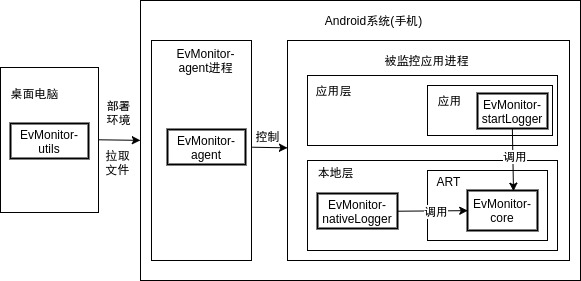
\includegraphics[width=\textwidth]{em_overview.jpg}
	\caption{EvMonitor概览}
	\label{emOverview}
\end{figure}

下面的内容从系统的配置和控制\dunhao 监控应用启动\dunhao 监控Java方法调用\dunhao 监控本地函数调用\dunhao 脱壳功能和日志系统功能方面介绍了应用的实现原理\juhao
\section{系统的配置和控制}
本功能由EvMonitor\_agent实现\juhao EvMonitor\_agent启动后开启域套接字(Linux系统的一种进程间通信机制)监听/data/local/tmp/EvMonitor/sock路径, 并开启一个线程用来接收用户指令发送到各个被监控的应用进程\juhao 当被监控的应用启动时, 其每个进程都通过域套接字连接到EvMonitor\_agent\juhao 在每个进程连接时, EvMonitor\_agent读取并解析配置文件将结果发送到目标进程, 并记录此连接的文件描述符用于之后发送用户指令, 然后开启一个线程来监控此连接的状态\juhao 当被监控应用的某个进程退出时, 监控该进程连接状态的线程会将记录此进程与EvMonitor\_agent连接的文件描述符删除\juhao 用户输入指令时, 接收用户指令的线程会读取用户输入的指令并通过记录的文件描述符发送给被监控应用运行中的每个进程\juhao 

\section{监控应用启动}
本功能由EvMonitor\_startLogger实现\juhao 
\ref{appStartA}节详细介绍了Android系统应用的启动过程\juhao 由于Android应用进程不是通过直接使用应用APK文件启动, 而是通过Zygote进程fork产生, 因此无法按照传统PC上启动子进程, 然后加载监控模块开启监控, 最后再加载目标应用开始执行的方式来实现在应用加载前启动对应用的监控\juhao 只有通过监控应用的启动, 在能够获取到应用的名称并且应用自身代码还未执行时开启完成监控应用的初始化操作\juhao ActivityThread类的handleBindApplication方法开始的位置符合上述条件, 因此本系统选择在handleBindApplication方法的适当位置添加监控代码\juhao 

监控代码的实现逻辑如下:
首先读取当前进程名和应用名(有些应用会启动多个进程), 使用日志系统记录当前启动的应用名和进程名\juhao 接着读取系统属性em.target\_type, 确定是只监控某个进程还是监控该应用的全部进程\juhao 接着根据上述结果读取系统属性获取要监控的进程名或者应用名并同本进程或者应用名比较, 如果不同则退出监控代码, 不启动监控系统; 如果相同则调用Evmonitor-core提供的初始化监控的接口来启动对该应用的监控\juhao 之后再根据当前运行环境是32位还是64位加载对应的EvMonitor-Frida动态链接库, 完成监控系统的初始化\juhao 

为了便于调用JNI和被调用, 我将上述监控代码作为一个新的静态方法logAppStartAndSetTarget\_em加入了com.android.internal.os.Zygote类中, 并通过在Zygote类中增加本地方法nativeEnableMonitor的方式调用了EvMonitor-core提供的本地层接口\juhao 

\section{监控Java方法调用}
本功能由EvMonitor\_core实现\juhao 
为了能够获取到应用所有Java方法调用行为, 本系统选择在ART内执行方法的函数中加入监控代码\juhao  \ref{methodExecA}节详细介绍了ART虚拟机执行方法的过程\juhao 根据分析, 在ArtMethod::Invoke和Execute函数中插入监控代码就能够记录所有的Java方法调用情况\juhao  

ART虚拟机中的每个Java方法都使用一个ArtMethod类型的对象来表示, 而在ArtMethod::Invoke和Execute执行方法时都能够获取到代表正在执行的方法的ArtMethod对象, 因此本系统在ArtMethod类(/art/runtime/artmethod.cc)中加入一个方法log\_em用于记录当前方法并写入日志中\juhao log\_em方法会调用当前ArtMethod对象的PrettyMethod方法获取方法信息然后调用EvMonitor-core中的日志系统将其写入日志\juhao 

本系统在ArtMethod::Invoke和Execute函数的入口和所有出口位置调用了上述log\_em函数记录方法执行的开始和结束\juhao 

\section{监控本地函数调用}
本功能由EvMonitor\_nativeLogger实现\juhao 本系统使用Frida工具的动态链接库形式(frida-gadget), 通过在应用加载自身代码之前加载frida-gadget并执行监控代码来实现对本地层函数调用的监控\juhao 目前的监控较为简单, 主要是利用了Frida工具提供的Interceptor来hook了open\dunhao execve\dunhao connect\dunhao dlsym函数来监控它们的调用情况\juhao 由于Frida工具实现了Javascript的API, 因此可以通过脚本文件灵活的添加监控函数和其他监控逻辑, 增强本系统\juhao 


\section{脱壳功能}
本功能由EvMonitor\_core实现\juhao 
目前Android平台应用加固工具的加壳机制十分复杂, 本系统根据\ref{classLoadA}节介绍的类加载过程, 通过在用于dex文件加载的关键函数, 即位于安卓源代码中/art/runtime/DexFile.cc中DexFile类的构造函数DexFile()中加入代码来实现简单脱壳获取dex文件的功能\juhao 
DexFile类的构造函数原型图\ref{dexFileCode}所示\juhao 
\begin{figure}[ht]
	\centering
	\fbox{
\includegraphics[width=8cm]{dex_file_code.jpg}}
	\caption{DexFile()原型}
	\label{dexFileCode}
\end{figure}
其中第一个参数是dex文件被加载到内存的起始地址, 第二个dex文件的大小\juhao 本系统插入该函数的监控代码会先检查是否开启对当前进程的监控, 如果监控功能没有开启则不在执行后续操作\juhao 如果监控功能开启会先调用日志系统记录当前加载的dex文件起始地址和大小, 然后再检查是否启动脱壳功能\juhao 如果脱壳功能启动则读取这两个参数后会调用EvMonitor\_core中用于保存dex文件的dumpDex函数, 将加载的dex文件写入配置文件设定的位置\juhao 


\section{日志系统}
本功能由EvMonitor\_core实现\juhao 各种动态分析系统中, 输出监控记录都是一个十分重要的功能, 但由于IO的速度很慢, 在频繁的调用中记录日志信息对应用本身的执行速度影响很大\juhao 在最初的测试中本系统使用Android系统本身的日志系统接口来记录监控信息, 但在测试中发现Java层方法的调用很多, 通过Android系统本身的日志系统输出会导致应用运行变得非常慢, 所以开发了本系统的日志部分\juhao 

表\ref{logValue}描述了日志系统用到的一些变量和提供的接口函数\juhao 
% Please add the following required packages to your document preamble:
% \usepackage{multirow}
\begin{table}[ht]
	\centering
	\caption{日志系统变量和函数}
	\begin{tabular}{cll}
		\hline
		\multicolumn{1}{l}{}                             & \textbf{名称}       & \textbf{作用}     \\ \hline
		\multirow{4}{*}{\textbf{变量}}                     & log\_base         & 记录日志缓冲区起始地址     \\
		& log\_data         & 记录日志缓冲区空闲区起始地址  \\
		& log\_spare\_space & 记录日志缓冲区空闲空间     \\
		& log\_file\_amount & 记录已经写入磁盘的日志文件数量 \\ \hline
		\multicolumn{1}{l}{\multirow{2}{*}{\textbf{函数}}} & log()             & 写入日志            \\
		\multicolumn{1}{l}{}                             & writeLog()        & 把缓冲区日志写入文件      \\ \hline
	\end{tabular}
\label{logValue}
\end{table}
日志系统会在初始化时使用mmap创建一个4M的内存缓冲区, 并在被监控应用的目录下以当前进程号创建一个文件夹用来保存此次执行时的日志数据\juhao 缓冲区的起始地址会使用log\_base来记录, 并且log\_data会被初始化为同log\_base一致\juhao 

log函数被调用来记录日志时, 会先检查log\_spare\_space, 如果空间足够就会把接收到的日志信息加上当前线程号写入log\_data位置处的内存缓冲区中并更新log\_spare\_space\dunhao log\_data的值 \juhao 如果空间不足就会调用writeLog函数试图把缓冲区的日志写入文件\juhao writeLog函数会检查log\_file\_amount的值确定日志文件数量是否达到最大, 如果是, 则通过Android系统的log系统记录一个日志文件以达到数量上限的错误, 并不在执行后续操作, 如果不是则将缓冲区的数据写入文件, 并将log\_base的值赋给log\_data, 设置log\_spare\_space的值为缓冲区最大容量, 同时把log\_file\_amount加1\juhao 


\chapter{实验与结果分析}
\section{实验总体方案}
本系统的测试分为两个部分, 第一部分是功能测试, 第二部分是性能测试\juhao 功能测试部分主要测试监控应用启动, 监控Java方法调动, 监控本地函数执行以及脱壳功能是否正常运行, 结果是否准确; 性能测试部分主要测试在监控系统运行时的性能开销, 并同Android Device Monitor做对比测试\juhao 
\section{实验运行环境}
由于本系统基于Android8.1构建, 并运行于真机上, 因此本次实验会涉及两台设备\juhao 设备1是用于配置和控制本系统的个人电脑, 设备2是运行该系统的智能手机, 两台设备的硬件和软件环境如表\ref{environment}所示\juhao

\begin{table}[ht]
	\centering
	\caption{实验设备环境}
	\resizebox{\textwidth}{!}{%
		\begin{tabular}{lllll}
			\hline
			设备                               & 型号                       & \textbf{CPU(型号/主频)}           & \textbf{内存} & 操作系统         \\ \hline
			\multicolumn{1}{c}{\textbf{设备1}} & Lenovo XiaoXin 700-15ISK & Intel core i5 6300HQ / 2.3GHZ & 8GB         & 深度操作系统15.9.3 \\ \hline
			\textbf{设备2}                     & Google Nexus 5X          & MSM8992 / 1.8GHZ              & 2GB         & Android8.1   \\ \hline
		\end{tabular}%
	}
	\label{environment}
\end{table}
\section{功能测试}
本次功能测试使用了支付宝应用的10.1.62版本(应用软件包名com.eg.android.\\AlipayGphone)本文作者开发的一款名为noticer的应用(应用软件包名top.january147\\.noticer)来进行\juhao noticer应用经过360加固保\upcite{360jiagubao}加固, 以检测本系统功能的有效性\juhao 
\subsection{监控应用启动功能测试}
在设备1上开启终端, 输入adb logcat|grep EvMonitor等待读取本系统监控应用启动的记录\juhao 然后执行如下操作:在设备2上启动支付宝应用, 然后退出支付宝应用再启动noticer应用\juhao

从终端中读取的监控记录如图\ref{testAppStart1}所示\juhao
\begin{figure}[ht]
	\centering
	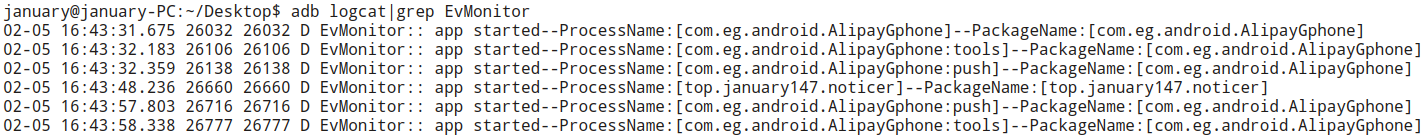
\includegraphics[width=\textwidth]{test_app_start_1.png}
	\caption{应用启动监控记录}
	\label{testAppStart1}
\end{figure}
监控记录显示支付宝应用的首先启动, 该应用共计启动了3个进程, 进程名分别为com.eg.android.AlipayGphone\dunhao com.eg.a-ndroid.AlipayGphone:push\dunhao 和com.eg.android.AlipayGphone:tools; 接着记录了noticer的启动, 该应用只启动了一个进程, 进程名为top.january147.noticer; 后边又记录了支付宝启动的两个进程,com.eg.android.AlipayGphone:tools和com.eg.android.A-lipayGphone:push而测试流程中并没有再次执行支付宝, 可以看到支付宝有自动启动的行为\juhao 

\subsection{监控Java方法调用功能测试}
\label{testJavacallA}
在设备1上开启终端, 键入adb shell进入设备2的shell\juhao 此时利用setprop命令设置系统属性em.target\_app为noticer软件的包名top.january147.noticer, 然后再执行logcat | grep Evmonitor查看系统运行情况\juhao 在设备2上启动noticer, 启动后界面如图\ref{testNoticer}所示, 点击底部的电话通知服务按钮启动电话通知服务, 等待启动完成再次点击该按钮关闭电话通知服务, 完成后退出应用\juhao 此时在设备1上运行脚本pull\_log\_dir.sh获取目标应用日志文件夹\juhao
\begin{figure}[ht]
	\centering
	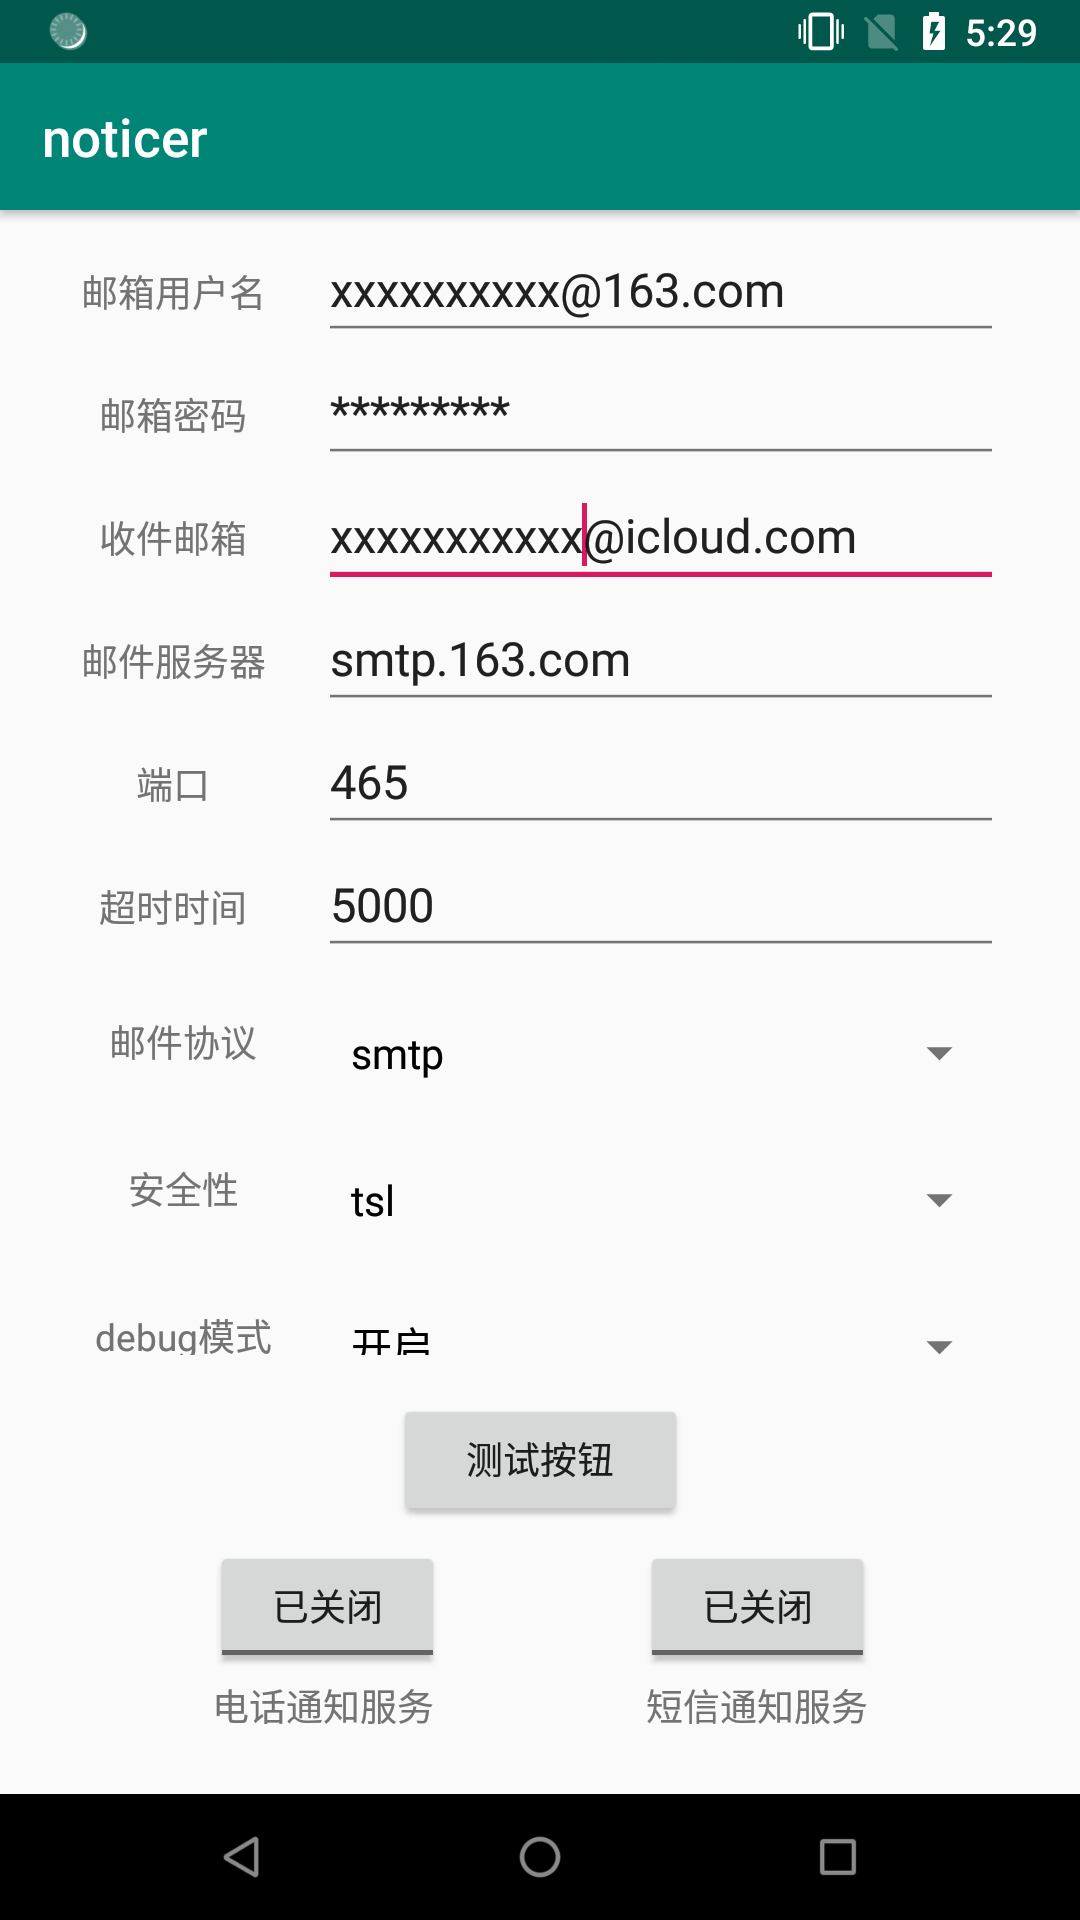
\includegraphics[width=4cm]{test_noticer.png}
	\caption{noticer界面}
	\label{testNoticer}
\end{figure}

图\ref{testJavacall}是终端中显示的本系统的运行信息\juhao 可以看到, 应用启动监控模块检测到目标应用启动后调用本地层的接口进行了一系列初始化操作, 包括创建日志文件夹, 分配日志缓冲区等等, 此外还记录了dex文件解析的情况\juhao 
\begin{figure}[ht]
	\centering
	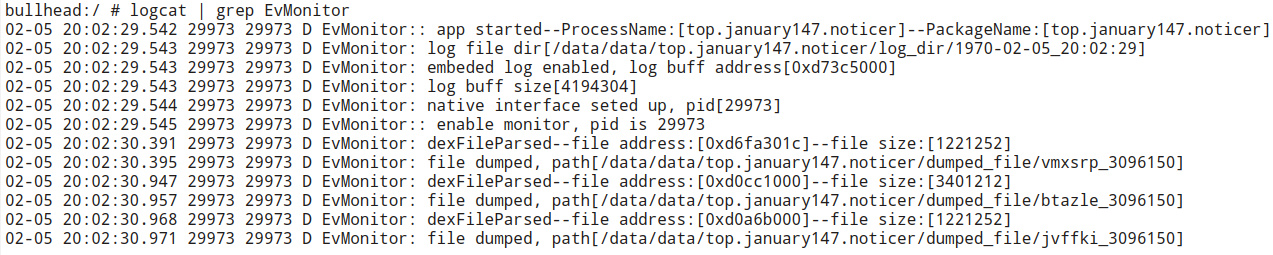
\includegraphics[width=\textwidth]{test_javacall.png}
	\caption{监控系统运行日志}
	\label{testJavacall}
\end{figure}

打开脚本pull\_log\_dir.sh从目标应用目录下取得的日志文件夹会发现一个以时间命名的文件夹, 该文件夹记录了应用在上述执行过程中的日志数据, 其文件如图\ref{testLogFile}所示\juhao 可以看到有许多em\_开头后接数字编号编号的log文件, 编号即为log文件生成的顺序, 这些文件记录了应用在上述过程执行中全部Java方法调用\juhao 
\begin{figure}[ht]
	\centering
	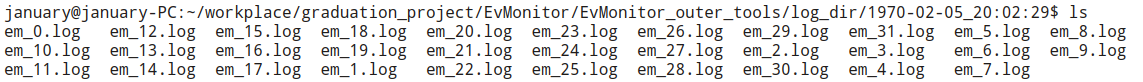
\includegraphics[width=\textwidth]{test_log_file.png}
	\caption{Java调用记录日志文件}
	\label{testLogFile}
\end{figure}

限于论文篇幅原因, 本文使用脚本log\_filter.sh过滤上述日志文件, 生成只包含noticer自身方法调用的记录文件, 并在其中搜索关于执行应用运行时两次点击按钮的调用记录, 结果如图\ref{testServiceStart}和\ref{testServiceStop}所示\juhao 由于启动服务需要进行许多初始化操作, 流程较长图\ref{testServiceStart}是服务启动开始时和完成时的部分调用记录\juhao 图\ref{testServiceStart}是关闭服务的完整调用记录\juhao 每条记录的格式为"线程号 执行方式 方法名称", 执行方式由两个大写字母和"--"组成, 第一个字母为I表示方法开始执行, 为O表示方法执行结束; 第二个字母为V表示通过ArtMethod::Invoke函数执行, 为E表示通过Execute函数执行\juhao 
\begin{figure}[ht]
	\centering
	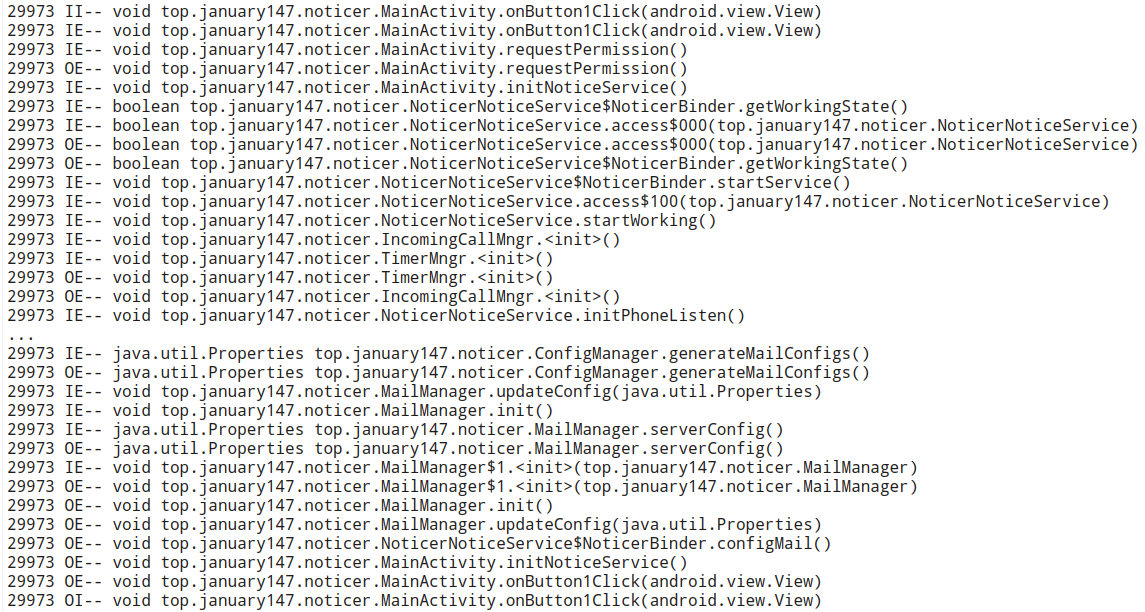
\includegraphics[width=\textwidth]{test_service_start.png}
	\caption{启动电话通知服务的调用记录}
	\label{testServiceStart}
\end{figure}
\begin{figure}[ht]
	\centering
	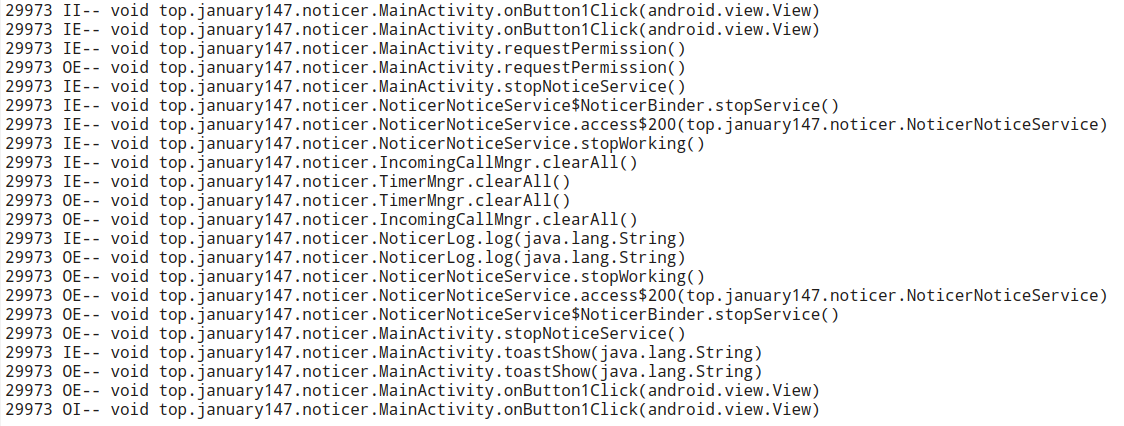
\includegraphics[width=\textwidth]{test_service_stop.png}
	\caption{关闭电话通知服务的调用记录}
	\label{testServiceStop}
\end{figure}

\subsection{脱壳功能测试}
\ref{testJavacallA}小节测试流程中本系统已经启动并执行了脱壳功能, 在本小节的测试中直接使用脚本pull\_dumped\_file.sh从目标应用文件夹获取得到包含dex文件的文件夹\juhao 该文件夹中为3个dex文件, 使用dex2jar工具转换成jar文件后文件夹内容如图\ref{testDexFile}所示\juhao 没有后缀名的3个文件为脱壳工具抓取的dex文件, 其他3个为dex2jar工具转换后对应的jar文件\juhao 
\begin{figure}[ht]
	\centering
	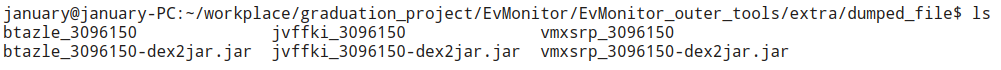
\includegraphics[width=\textwidth]{test_dex_file.png}
	\caption{脱壳工具抓取的dex文件}
	\label{testDexFile}
\end{figure}

使用jd-gui打开3个jar文件后成功在名为btazle\_3096150-dex2jar.jar的文件中找到了实现应用真实功能的类, 成功实现了脱壳\juhao 图\ref{testOrgClass}是jd-gui工具查看的结果, top.january147.noticer包下的类即为应用本身的类, 右侧显示的为\ref{testJavacallA}小节中Java方法调用记录中的onButton1Click方法源代码\juhao 
\begin{figure}[ht]
	\centering
	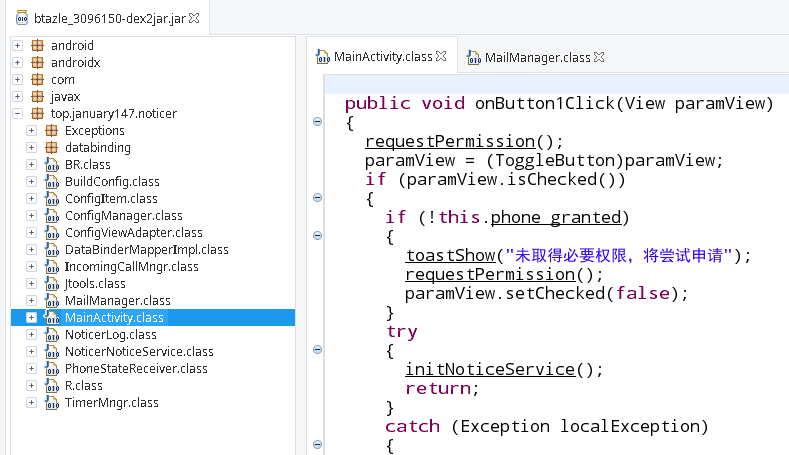
\includegraphics[width=\textwidth]{test_org_class.png}
	\caption{脱壳后得到应用本身的类}
	\label{testOrgClass}
\end{figure}

\subsection{监控本地函数调用功能测试}
开启监控目标应用noticer, 本系统记录的本地调用信息会保存到应用目录下的log\_dir文件夹中, 从中获取的本地函数调用信息如图\ref{testNativeCall}所示\juhao 
\begin{figure}[ht]
	\centering
	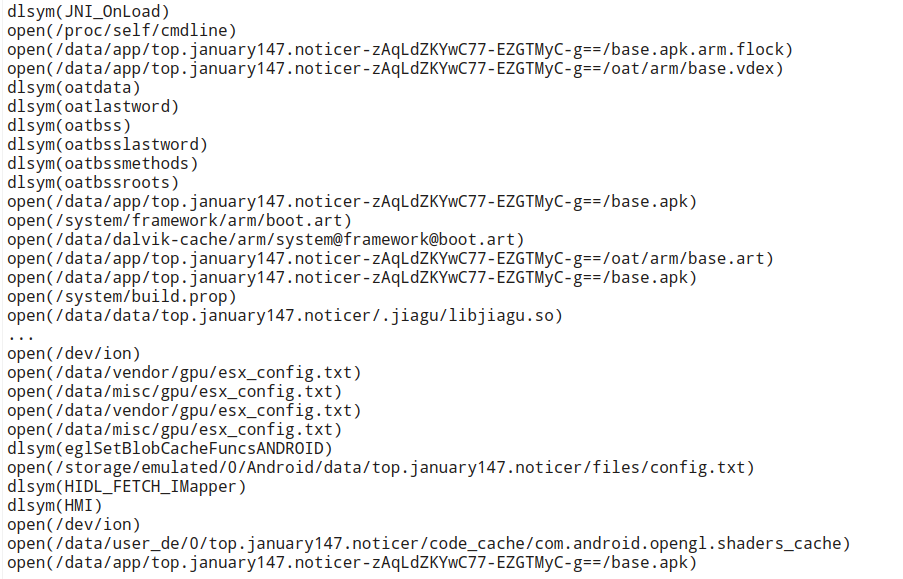
\includegraphics[width=\textwidth]{test_native_call.png}
	\caption{本地函数调用记录}
	\label{testNativeCall}
\end{figure}

\section{性能测试}
由于本系统的主要性能开销在于记录方法调用时的性能开销, 针对cpu性能的性能测试工具无法成功检测本系统的性能, 因此本文开发了一个简单的测试Java方法调用性能检测的应用, 该应用将一个简单的无内部调用的java方法执行固定次数并测量总用时用于评价Java方法调用性能\juhao 本文使用了该应用对本系统和Android Device Monitor的Method Profile功能进行了测试, 结果如图\ref{testOverhead}所示\juhao 
\begin{figure}[ht]
	\centering
	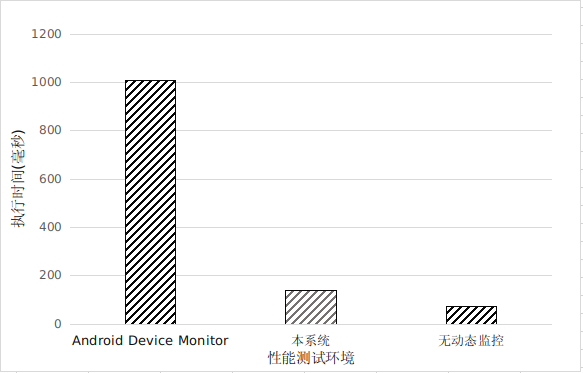
\includegraphics[width=8cm]{test_overhead.png}
	\caption{本地函数调用记录}
	\label{testOverhead}
\end{figure}
其中的执行时间为10次测量结果取平均值得到的\juhao

\section{结果分析}
功能测试的结果显示本系统的基本功能正常, 能够实现对应用启动\dunhao Java方法调用\dunhao 本地函数调用的监控和以及脱壳功能, 系统设计原理可行\juhao 性能测试的结果显示本系统的执行耗时约为正常执行时的两倍, 而Android Device Monitor执行耗时约为正常执行的14倍, 本系统为Android Device Monitor的Method Profile功能运行效率的7倍, 因此十分高效\juhao 


\chapter{总结与展望}
\section{论文工作总结}
Android平台的应用, 无论是正常的还是恶意的, 都在利用不断变化的技术来对抗应用分析, 然而对应用进行分析又是辨别出恶意应用比不可少的环节, 因此应用开发者想尽办法隐藏应用的真实行为, 应用分析者想尽办法找出应用隐藏的行为就成了一场持续的对抗\juhao 学习Android系统的设计原理和现有技术则是加入这场对抗十分重要的部分, 在充分理解已有知识的基础上, 才能产生新的知识\juhao 本文将主要工作重心放在学习Android系统和已有的动态分析技术上, 并在新的Android系统上进行了部分实践, 具体来说, 论文的主要工作内容如下:

	 研究了Android系统的整体架构, Android应用开发相关知识,  研究了国内外关于Android平台动态分析的多项技术成果并总结了对抗应用分析的常用技术和实现动态分析常用的技术和工具, 分析了其优势和劣势\juhao 
	 
	 深入源代码分析了Android8.1系统中ART虚拟机的设计和运行机制, 在3个重要方面, 即应用的启动\dunhao 类的加载和方法的执行方面给出了关键调用图\juhao 
	 
	 利用上述研究的成果设计和实现了一个Android应用的动态行为捕获系统, 并实现了简单的脱壳功能\juhao 对本文实现的系统进行了详细的测试, 验证了设计方案的可行性和有效性\juhao 
	 
\section{进一步工作展望}
本文对于Android系统, Andriod平台动态分析技术及其相关技术(如调试技术)的认识还不够深刻, 并且
本文所有构建的系统只是对设计思路的简单测试, 并不是一个成熟的高可用性的系统, 因此未来的
未来的工作分为两部分, 第一部分是继续深入研究和测试已有的调试技术和动态分析技术, 深入研究Android系统各个部分的设计和实现原理, 第二部分是完善本系统的设计和实现, 具体来说有以下方面:

本系统使用Frida框架对本地函数调用进行监控, 而Frida框架的稳定性不够好, hook某些函数如dlopen时会导致应用崩溃, 并且难以对所有的本地函数调用序列进行监控, 下一步计划使用ptrace系统调用来构建本地层的监控功能\juhao

本系统没有对监控到的Java方法的参数和返回值进行解析, 下一步计划加入解析参数和返回值的功能\juhao 

本系统产生的Java调用日志数量众多且不易阅读, 下一步计划加入有效的过滤机制减少日志数量输入更有效的日志记录\juhao 
	


\phantomsection
\addcontentsline{toc}{chapter}{参考文献} %将“参考文献加入目录中”
\bibliography{ref}


\backmatter
% !Mode:: "TeX:UTF-8"
%%%%%%%%%%%%%%%%%%%%%%%%%%%%-------致谢--------%%%%%%%%%%%%%%%%%%%%%%%%%%%%%%%%

\acknowledgement
\addcontentsline{toc}{chapter}{致谢}















\cleardoublepage
\end{document}



